\subsection{طراحی سیستم و نرم افزار}
طراحی های کلی نرم افزار در مقدمه و مشخص سازی خواسته ها صحبت شده. الباقی کار نیازمند مشخص سازی و طراحی تیم فنی است. این مستندات از تیم فنی بعد از 
برگزاری جلسات معماری اخز شده و بایگانی می‌شود.
مستندات مربوط به معماری پیاده سازی حدالامکان نباید تغییر کند.

\subsubsection{نمودار DFD پروژه}

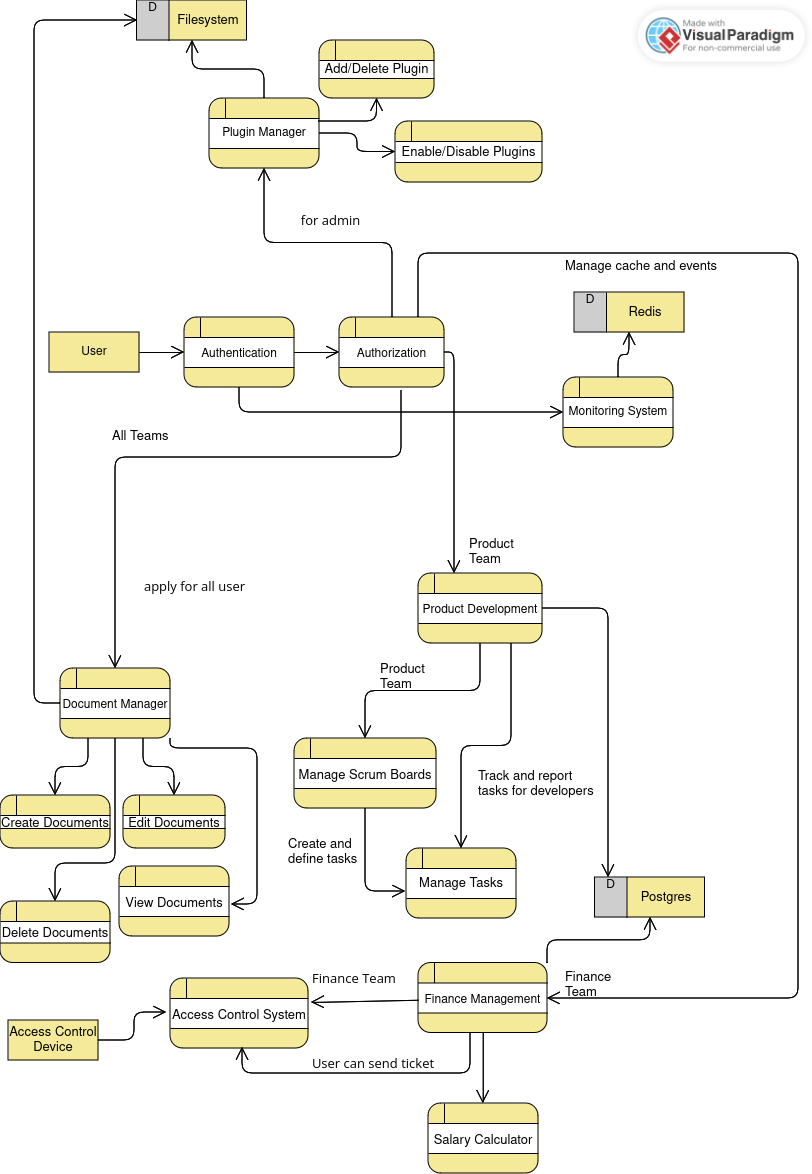
\includegraphics[scale=0.55]{assets/main_dfd.png}

کلیات و جریان داده های پروژه در نمودار DFD پروژه بیان شده.

\subsubsection{نمودار ERD پروژه}

توجه کنید که نمودار ER زیر بر اساس استاندارد علامت گذاری Chen است. سمبل های امروزی از مدل های دیگری برای نمایش موجودیت ها و روابط بینشان استفاده می‌شود.
اما سمبل ها و شیوه رسم نمودار زیر بر اساس علامت گذاری چن می‌باشد.

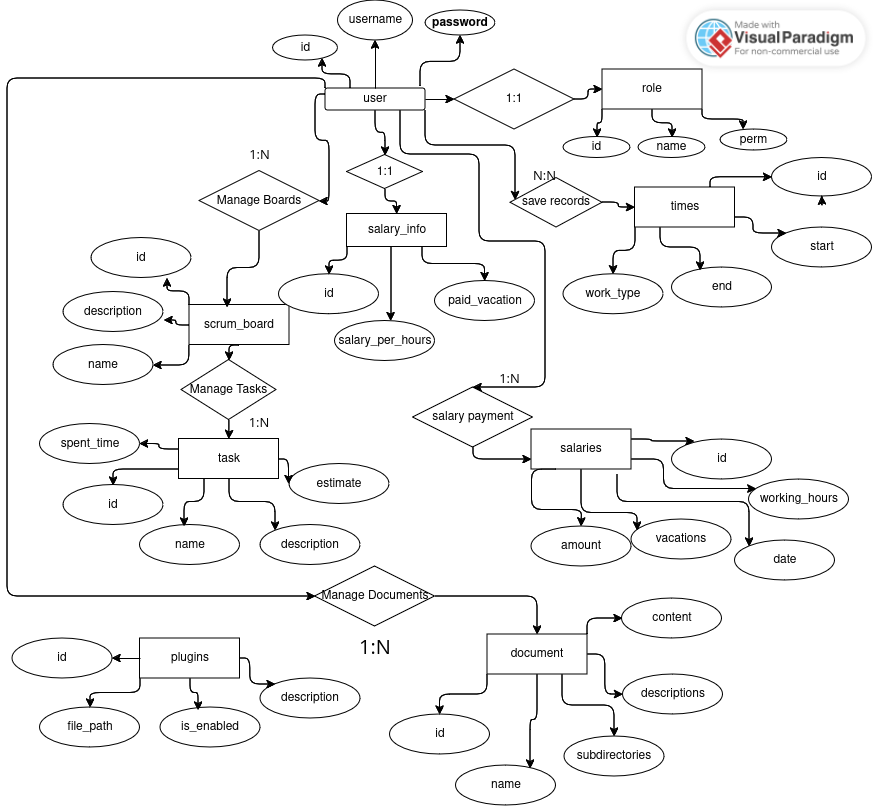
\includegraphics[scale=0.6]{assets/main_erd.png}
